\documentclass[a4j]{jarticle}
%\documentclass{jarticle}
\usepackage{conf_jst}
\usepackage{graphicx}
\usepackage{multirow}
\usepackage{listings}
\usepackage{plistings}
%\usepackage{fancyheadings}
\usepackage{longtable}
\usepackage{booktabs}

\oddsidemargin -10mm % 15mm - 1inch(25.4mm)
\evensidemargin -10mm
\textwidth 180mm  % A4幅210mm - 15*2mm
%\topmargin -10.4mm % 25mm - 25.4
\topmargin -10mm % 25mm - 25.4
\textheight 257mm % A4高さ297mm - 25*2mm
%\headheight 10mm
%\headsep 10mm

\setcounter{figure}{0}              %ここで図番号の変更が行えます.
\setcounter{table}{0}               %ここで表番号の変更が行えます.
\setcounter{equation}{0}            %ここで式番号の変更が行えます.

\if0
\def\thefigure{\thesection\arabic{figure}}      %図番号の形式設定
\def\thetable{\thesection\arabic{table}}        %表番号の形式設定
\def\theequation{\thesection\arabic{equation}}  %数式番号の形式設定
\fi

\setkeys{Gin}{width=7.0cm}  % 図のデフォルトサイズ

\pagestyle{plain}

% \longtableをtwocolumn環境で使えるようにする
\makeatletter
\let\oldlt\longtable
\let\endoldlt\endlongtable
\def\longtable{\@ifnextchar[\longtable@i \longtable@ii}
\def\longtable@i[#1]{\begin{figure}[htbp]
\onecolumn
\begin{minipage}{0.5\textwidth}
\oldlt[#1]
}
\def\longtable@ii{\begin{figure}[htbp]
\onecolumn
\begin{minipage}{0.5\textwidth}
\oldlt
}
\def\endlongtable{\endoldlt
\end{minipage}
\twocolumn
\end{figure}}
\makeatother

\title{2020/03/10 研究報告資料}
\author{氏名:田村 玄}
\date{期間:2019/11/15 ~ 2020/03/22}

\begin{document}
\maketitle

\section{これはセクションテストです}

hoge

\subsection{これはサブセクションテストです}

hoge

\subsubsection{これはサブサブセクションのテストです}

piyo

図の挿入テスト

\begin{figure}
\centering
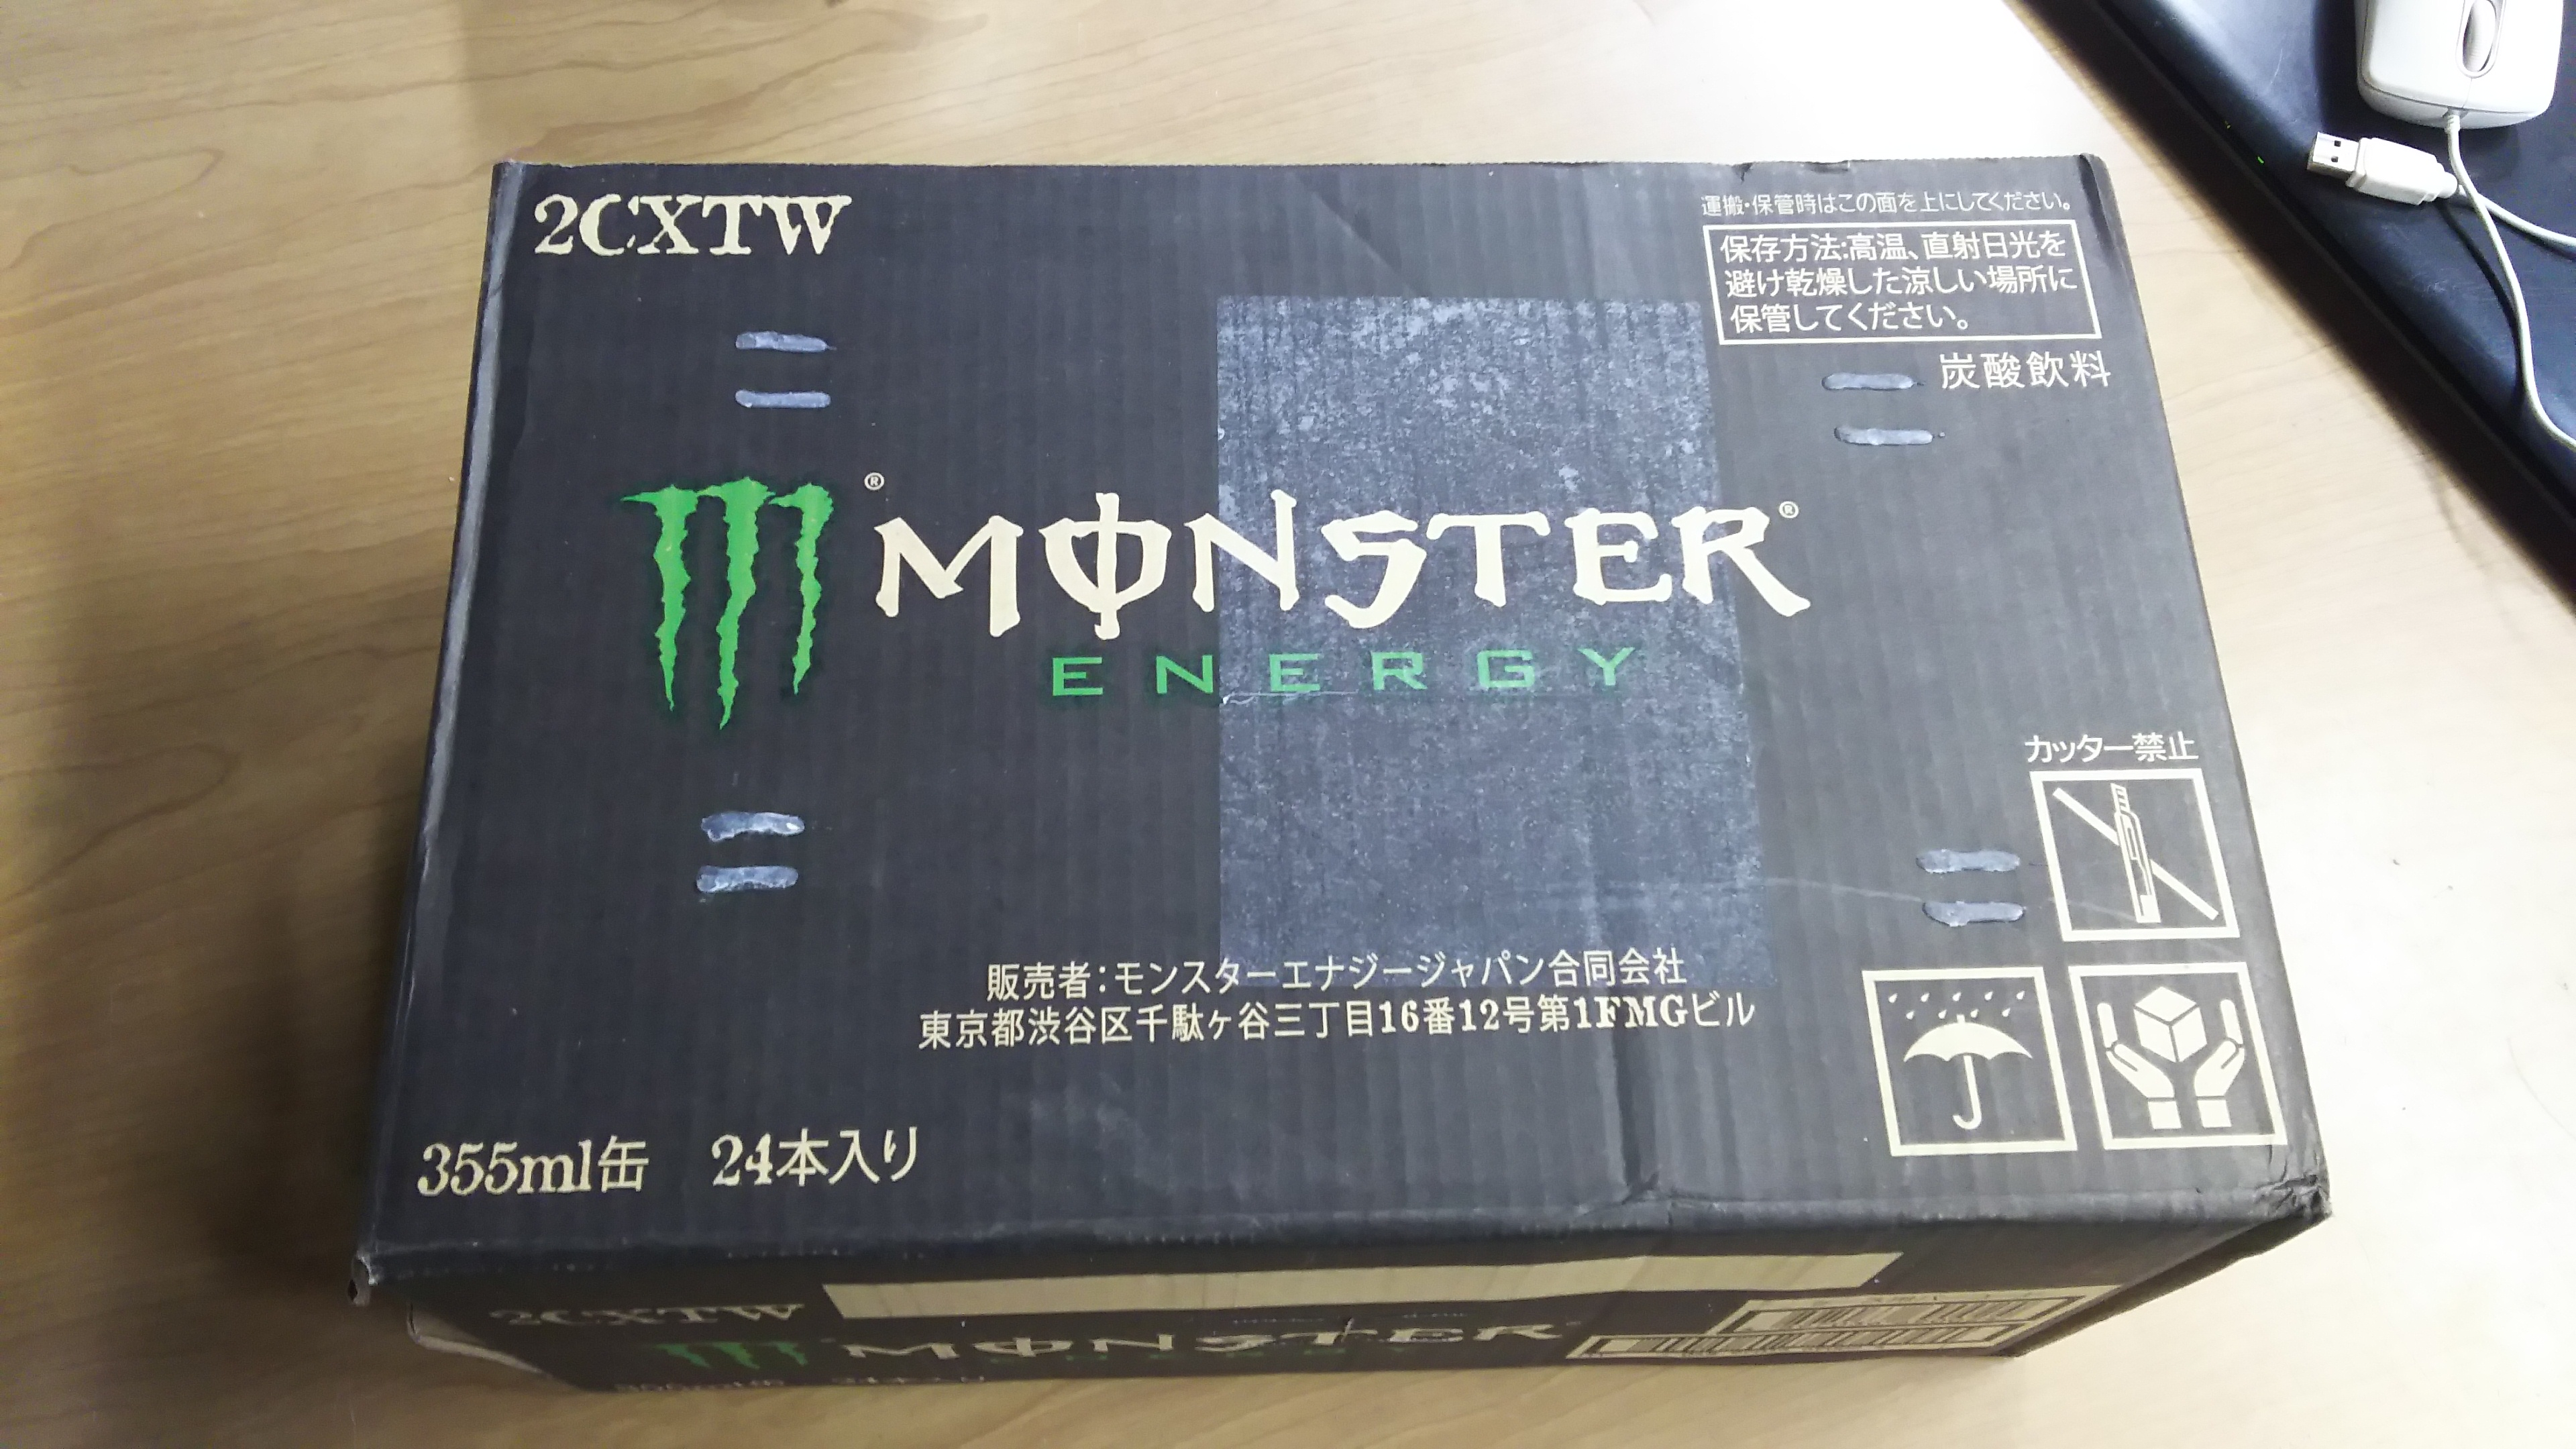
\includegraphics{DSC_0358.eps}
\caption{モンスターエナジー}
\end{figure}

もう一つ図を挿入

\begin{figure}
\centering

\includegraphics{end.eps}
\caption{はい終わり素子が逝った}
\end{figure}

表の挿入テスト

\begin{longtable}[]{@{}rllc@{}}
\toprule
右寄せ & 左寄せ & デフォルト & 中央寄せ\tabularnewline
\midrule
\endhead
12 & 12 & 12 & 12\tabularnewline
123 & 123 & 123 & 123\tabularnewline
1 & 1 & 1 & 1\tabularnewline
\bottomrule
\end{longtable}

\end{document}
